\chapter{Pacote ROS (cliente)}

Como já foi mencionado anteriormente o cliente é um pacote ROS, sendo assim, deve-se levar em consideração, os conceitos de programação do framework ROS em seu desenvolvimento. As técnicas específicas de programação ROS usadas no cliente serão descritas com detalhes neste capítulo, além da explicação do seu funcionamento interno e do uso da libinterfacesocket.

No desenvolvimento de aplicações com ROS deve ser respeitada a estrutura de diretórios  de um pacote ROS\@. Pacotes são a maneira com que os softwares são organizados no ROS, eles podem conter desde nós, que são a unidades de processamento do ROS, até mesmo bibliotecas ou módulos de softwares de terceiros. Os pacotes devem seguir uma estrutura padrão, por este motivo o código fonte do cliente foi organizado como é mostrado na Imagem~\ref{fig:clientdiretorios} abaixo.

\begin{figure}[ht]
	\caption{Estrutura de diretórios pacote cliente}
	\begin{center}
		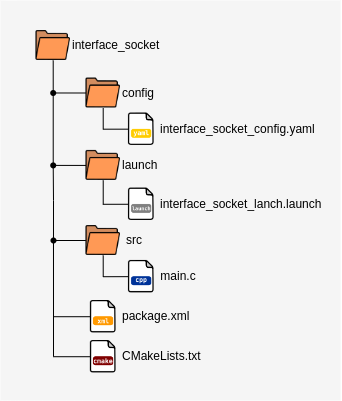
\includegraphics[scale=0.47]{imagens/rospackage.png}\\
		{\small \textbf{Fonte:} do autor}
    \end{center}\label{fig:clientdiretorios}
\end{figure}

A seguir será apresentada uma breve descrição de cada item do pacote:
 
\textbf{config/interface\underline{\hspace{.07in}}socket\underline{\hspace{.07in}}config.yaml:} Arquivo com o qual o usuário pode mudar alguns parâmetros de configuração da comunicação, como IP do servidor ou alguns outros parâmetros do tópico que será lido. Essa mudança pode ocorrer sem a necessidade de recompilar o código fonte, isso pode dar flexibilidade ao usuário do pacote durante o desenvolvimento de uma nova aplicação, que poderá ser configurada sem alterações no código fonte do nó. 

\textbf{launch/interface\underline{\hspace{.07in}}socket.launch:} Arquivo responsável chamar a execução do nó, além de carregar os parâmetros presentes no arquivo config.yaml no servidor de parâmetro do ROS\@.

\textbf{src/main.cpp:} Código fonte do executável, ou seja, o código fonte do único nó deste pacote.

\textbf{package.xml:} Manifesto do pacote é o arquivo que define as propriedades do pacote, como por exemplo, nome do pacote, autor, e dependências. Deve estar presente em todos os pacotes ROS~\cite{RosPkgXml}.


\textbf{CmakeLists.txt:} Contém instruções e diretivas para configuração do processo de compilação do pacote.

Este pacote disponibiliza apenas um executável, ou seja, apenas um nó que tem a finalidade de ler um tópico, enviar através da interface de rede os dados brutos contidos na mensagem do tópico de entrada, receber de volta esses dados processados pelo servidor, montar uma mensagem ROS e publicar essa mensagem através do tópico de saída. O processo descrito anteriormente é relativamente simples, como pode ser visto no fluxograma simplificado da Figura~\ref{fig:clientfluxo}

Este pacote disponibiliza apenas um executável, ou seja, apenas um nó que tem a finalidade de ler um tópico, enviar através da interface de rede os dados brutos contidos na mensagem do tópico de entrada, receber de volta esses dados processados pelo servidor, montar uma mensagem ROS e publicar essa mensagem através do tópico de saída. O processo descrito anteriormente é relativamente simples, como pode ser visto no fluxograma simplificado da Figura~\ref{fig:clientfluxo}

\begin{figure}[ht]
	\caption{Fluxograma pacote cliente}
	\begin{center}
		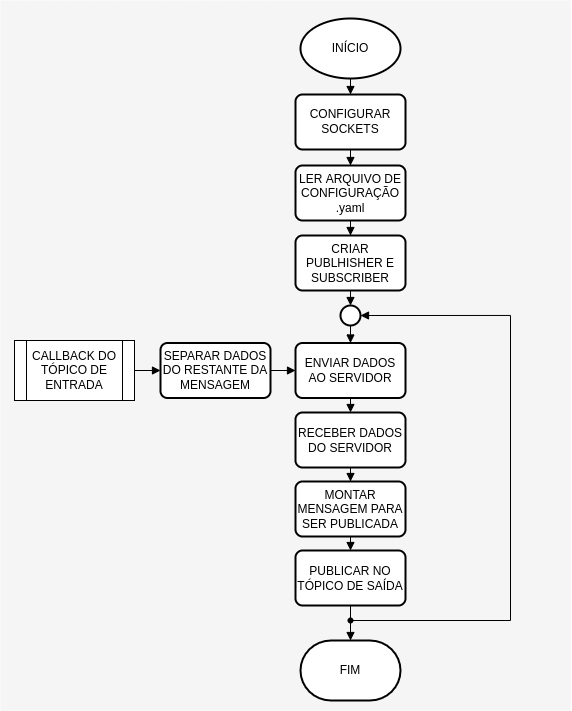
\includegraphics[scale=0.47]{imagens/fluxogramaCliente.png}\\
		{\small \textbf{Fonte:} do autor}
    \end{center}\label{fig:clientfluxo}
\end{figure}

Existem alternativas prontas para fazê-lo, como por exemplo o ROS serial, pacote ROS desenvolvido para permitir comunicação entre o ROS e outros dispositivos que possuem uma porta serial ou uma interface de rede [8]. A escolha por desenvolver um novo pacote para executar a mesma função se fez necessário pela necessidade de alta taxa de transferência de dados entre o ROS e o SoC para que seja aceitável a utilização do SoC com a finalidade de acelerar o processamento por hardware. Desenvolvendo um novo pacote de comunicação podemos extrair o máximo de desempenho da rede, como por  xemplo, escolhendo o melhor protocolo (UDP ou TCP) e transferindo apenas os dados para o processamento da informação. Todos os códigos do cliente podem ser encontrados no repositório disponível em [9].
